% Chapter 6

\chapter{Automated Reconfiguration}
\label{Chapter 6}
%\head{}

% 1 . Overview - what is the purpose of an agent?
\section{Overview}
This chapter discusses automated network reconfiguration and how it is supported by the work of this thesis. First, the concept of automated reconfiguration and the motivation for its use is described. Then the design and implementation of the automated reconfiguration software in the work of this thesis is described. Finally, an example is shown that demonstrates the practical uses of this software as a proof of concept.

% 2. Design 
%	- describe automated user & message processor 
%	- message processor is what distinguishes one agent from another 
%		- message processor can be made with a lambda and passed around as a first-class object (treating a function as a variable)
%		- cite this concept of lambda as a first class object
%	- the need to validate and separate permission checking from the automated user
%		- provides the motivation for a agentController
%	- mention how automated user is using the same logic/code from earlier in the paper
%		- using the same command classes
%		- automation is a natural extension of the work in the previous chapters
%	- class diagram of how all the classes fit together

\section{Design}
The work in this thesis allows network reconfiguration through user interaction. User interaction can sometimes be inadequate because of slow response time, a lack of understanding of system behavior, or human error. Creating a system that can automatically respond to incoming sensor data (or calculations derived from incoming sensor data) by reconfiguring the network allows overcoming many of the limitations encountered by requiring user input. \\


% 1. Describe the automated user class and how it needs to support several things when new automated users are implemented:
% - be able to handle received messages and exceptions that may be encountered
% - be able to adhere to the user access and safety validations of the rest of the system
% NOT allow some automated users to overwrite the UAC and safety validation
% NOT directly interact with the database
The software applications designed in this work to autonomously monitor and reconfigure WiSARDs are called automated agents. Agents have three main requirements that they must fulfill. First, the agents must adhere to the user access and safety validations that govern the rest of the system. More specifically, the developers of automated agents should not be allowed to intentionally or unintentionally bypass, improperly implement, or override the security provisions. Second, they must be able to receive and handle data messages, including being able to handle software exceptions that may occur. Finally, the agents should be able to interact with the cyberinfrastructure using the WiSARD abstraction. For instance, the agent should be able to interact with the PostgreSQL database using the methods that the WiSARD class provides. \\

% 2. Describe solution where each requirement is matched with a solution 

% (re-order the requirements above so that the first one is the second to last. Validation stuff first because it flows better later)

% Describe solution where each requirement is matched with a solution

% * adhere to validations and prevent bypassing or overwriting those checks -> Solution is put that logic in a different class
% * Handle received messages and exceptions specific to the specific type of automated user and its subscriptions -> Solution is to provide a specific implementation of each per type of automated user
% * Not directly interact with the database -> solution is to interact through the previously described wisard class

% 3. This all fits together in a design where a controller class encapsulates much of the functionality that was described in the previous chapters: primarily validation and safety

% describe about how there is common code between different automated users (creating subscriptions and listening for messages). You frequently get code re-use through inheritence
% but describe how in this case the design was cleaner to use composition over inheritance. This pulls out the MessageProcessor and ErrorHandler interfaces.

% Finally the WiSARD class is used when processing messages to interact with the data of the system.

% Show a resulting UML class diagram of the design with the AutomatedUser class at the center

The automated agents are defined by a Java class designed to address these three requirements. The first requirement of preventing agents from circumventing system security is solved by separating the validation logic from the agent class. If the validation logic is external to the agent class, then agents will not be able to dictate their own security privileges. The second requirement of receiving and handling data streams and handling exceptions specific to each agent is solved by the design decision that each agent must be provided message handling logic and exception handling logic specific to each agent. The final requirement of preventing an agent from directly accessing the PostgreSQL database is solved by using the WiSARD class discussed in Chapter 5 as a means of interacting with the database.\\ 

To accommodate these solutions, an agent controller class is used that encapsulates much of the functionality described in the previous chapters, primarily validation and safety. The controller class will log in an agent, validate that it has sufficient privileges to access the data streams it uses, and then create an agent object. The agent class implements the Java runnable interface, that allows it to be put into a thread and executed. The design and implementation of the agents is generalized, so that there is common code from agent to agent. Every agent uses the same logic to listen for and handle incoming messages. Message processing and error logic that distinguishes one agent from another are passed to the agent as parameters in the form of lambda expressions. A lambda expression is an anonymous function.\\

Using inheritance in object-oriented software design is typically a good way to reuse code. Inheritance has been used extensively in the code described in the previous chapters. However, in the case of designing the automation behavior, using composition over inheritance resulted in a cleaner design. Composition is the object-oriented design concept where the functionality of an object is defined through the creation of member objects rather than through inheriting methods. This approach is accomplished with the use of two interfaces referred to as the Message Processor and the Error Handler. These interfaces are what allow the operational logic for each agent to be passed in as lambda expressions. Figure \ref{fig:automation_class_diagram} is a class diagram that shows how these classes are implemented using a composition approach.\\

\begin{figure}[H]
	\centering
	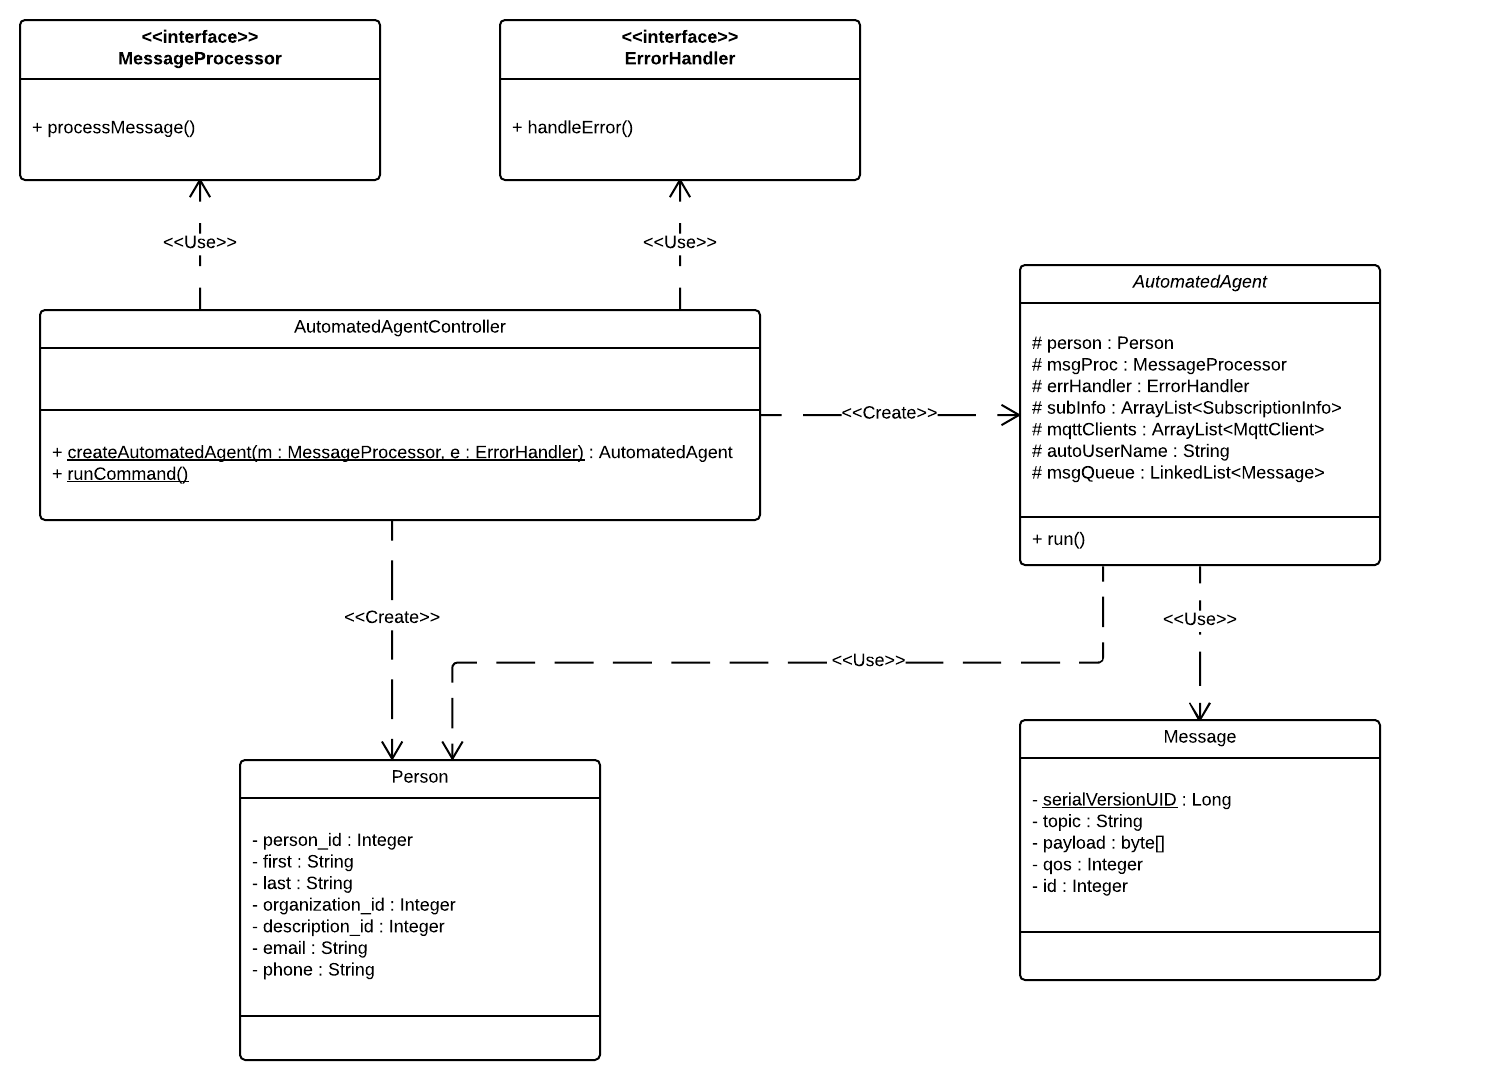
\includegraphics[width=\textwidth]{figures/automated_agent_class_diagram.png}
	\caption{A class diagram showing the composition of the agents and their relevant classes}
	\label{fig:automation_class_diagram}
\end{figure}

The text on each of the arrows denote a class using the item it is pointing to, or whether is is creating an instance of the item it is pointing to. The Automated User Controller class uses the Message Processor and Error Handler interfaces to create Automated User and Person objects. Each Automated User object can then use its Person object, the functionality in the Message class, and whatever functions that were passed in for the Message Processor and Error Handler to complete its tasks. A detailed example of the software classes showing how this software actually works is described in the next section.



%If a software application is given the data streams necessary to identify certain event conditions and the capability to make decisions, then the reconfiguration process can be automated, and performed in a quicker and more efficient way than if a human user were to do it. The Validation module and the user access control data schema work well for users and entities to perform reconfigurations. Because of this, designing an automated piece of reconfiguration software as an artificial user will allow the the reconfiguration to be governed by the same validation and user access control paradigm as human users.\\

%The software applications which autonomously monitor and reconfigure WiSARDs are called automated agents. It is important that these agents are designed an implemented in a way that respects the user access control paradigm so that they can safely and efficiently operate. Additionally, a modular approach to designing the agents is necessary to allow a wide variety of network management capabilities without being cumbersome to the developer.\\

% modular message processor
%The first piece of the automated agent is called the message processor. This component is responsible for acquiring data streams and fetching data so that the agent can analyze and make informed decisions. This component is the most modular piece of the automated agent, and is defined by a Java class whose objects are passed to the agent. The message processor in software is made using a Java 8 lambda expression, which allows it to be passed around as a first-class object \textbf{cite this}. 

%The message processor software can communicate with the PostgreSQL database as well as interact with MQTT brokers. This gives the developer the flexibility to access current data that has recently been sampled, but also lets the agents have access to archived data from the database for a diverse range of analyses. 

% agent uses same command and validation logic from previous chapter
%The second piece of the automated agent is the logic which generates commands to reconfigure WiSARDs based on whatever assessments resulted from the message processor. The flexible design of the Command Generation module allows the agent to utilize its functionality in the same way that a human user would be able. Additionally, the portion of the validation module which performs the safety validation checks can also be utilized by the agents in the same way that a human user can.\\


% need for validation and permission checking outside of the agent
%The user access control portion of the validation module is handled a bit differently than the safety validation check. Because users of the platform will eventually be creating their own agents, it is important for the user access validation to be checked separately, so that users will be less likely to exploit the permission system. This provides the motivation for a separate piece of software called the Automated Agent Controller.\\

%This piece of software is defined by a Java class which performs three functions. First, the controller takes in user login information as parameters. It logs in the user and verifies the identity of the automated agent against the permission entities in the database. Second, the controller looks at the message processor which it also is passed as a parameter. The controller validates that the user has sufficient privilege to access the data streams it will be monitoring. Finally, if the login and user access validations were successful, the controller will create an automated agent object. Once created, the agent object can run and autonomously manage the WiSARDs. 


% 6.3 Example Then just give the example code for MyAutomatedUser, AutomatedUser, and the interfaces

% Then end with a paragraph about how the design is good: it is simple and quick to create a user, it is flexible, etc...

\section{Example Agent}
% 3. Example description and code for a very simple agent
%	- flow of execution visual?%
Using the design described in the previous section, there are many different ways that an automated agent can be used to manage WiSARDs. The following code snippets and class definitions demonstrate how this functionality is used in practice.\\

Below is the class definition for the agent controller that handles authentication and creation of the agents.\\
% AutomatedUserController class
\lstinputlisting[language = java, firstline = 32, lastline=44]{AutomatedUser.java}
 
 
  This is the class definition for the agents. An instance of this class is created by the agent controller and returned. In the constructor, all of the necessary information to establish connections to MQTT message brokers as well as define the agent's behavior is passed in as a set of parameters. The run() method shows how an agent establishes its subscriptions with the MQTT brokers it will be listening to, and then waits for messages to arrive. Once messages arrive, they are given to the processMessage() method whose functionality was passed into the constructor as a lambda expression.\\
  
 % AutomatedUser class	
 \lstinputlisting[language = java, firstline = 64, lastline=132]{AutomatedUser.java}
 
 These are the definitions for the functional interfaces that allow lambda expressions to be passed to the agents to define their behavior.
 
 % Interfaces
 \lstinputlisting[language = java, firstline = 16, lastline=30]{AutomatedUser.java}
 
  This code snippet shows an example of how to utilize the classes defined above in a runnable program that uses automated agents. The comments demonstrate what code a user would need to add to customize their agent.\\ 	
 
 % using everything
 \lstinputlisting[language = java, firstline = 46, lastline=62]{AutomatedUser.java}
 

 	
%There are many different ways in which an automated agent can be used to manage WiSARDs in the WiSARDNet platform. For a practical example, assume a researcher desires to capture a set of high resolution soil moisture readings of rain events in a particular area, but does not want their WiSARD to sample at a high rate when there are no rain events. An automated agent could be used to identify pending storms from neighboring areas by monitoring their soil moisture data readings, and then preemptively updating the sampling rate of the WiSARDs at the region of interest.\\

%To create an automated agent with this functionality the steps described in the previous section need to be taken.

%\begin{itemize}
%	\item Define a Message Processor with the logic it will use to monitor the data streams of interest.
%	\item Create an ArrayList data structure of subscription objects with the connection information to the different sites it will be monitoring.
%	\item Create an Automated Agent Controller object
%	\item Use the Automated Agent Controller to create and authenticate an Automated Agent
%	\item Run the Automated agent.
%\end{itemize}

%\textbf{Show the code that defines a message processor}

%\textbf{Show the code that creates the arraylist of subscription objects as well as the class definition for subscription objects}

%\textbf{Show the code that creates the Automated Agent Controller and the Automated Agent as well as class definitions for both}

%\text{Show the code that runs the Agent and the logic it executes}